\section*{Überblick}

%\begin{figure}[htb]
%\begin{center}
%%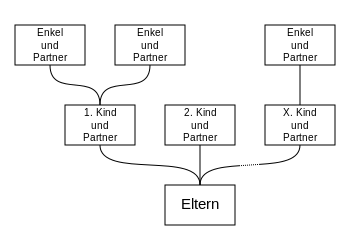
\includegraphics[width=.7\textwidth]{../fig/stammbaum.png}
%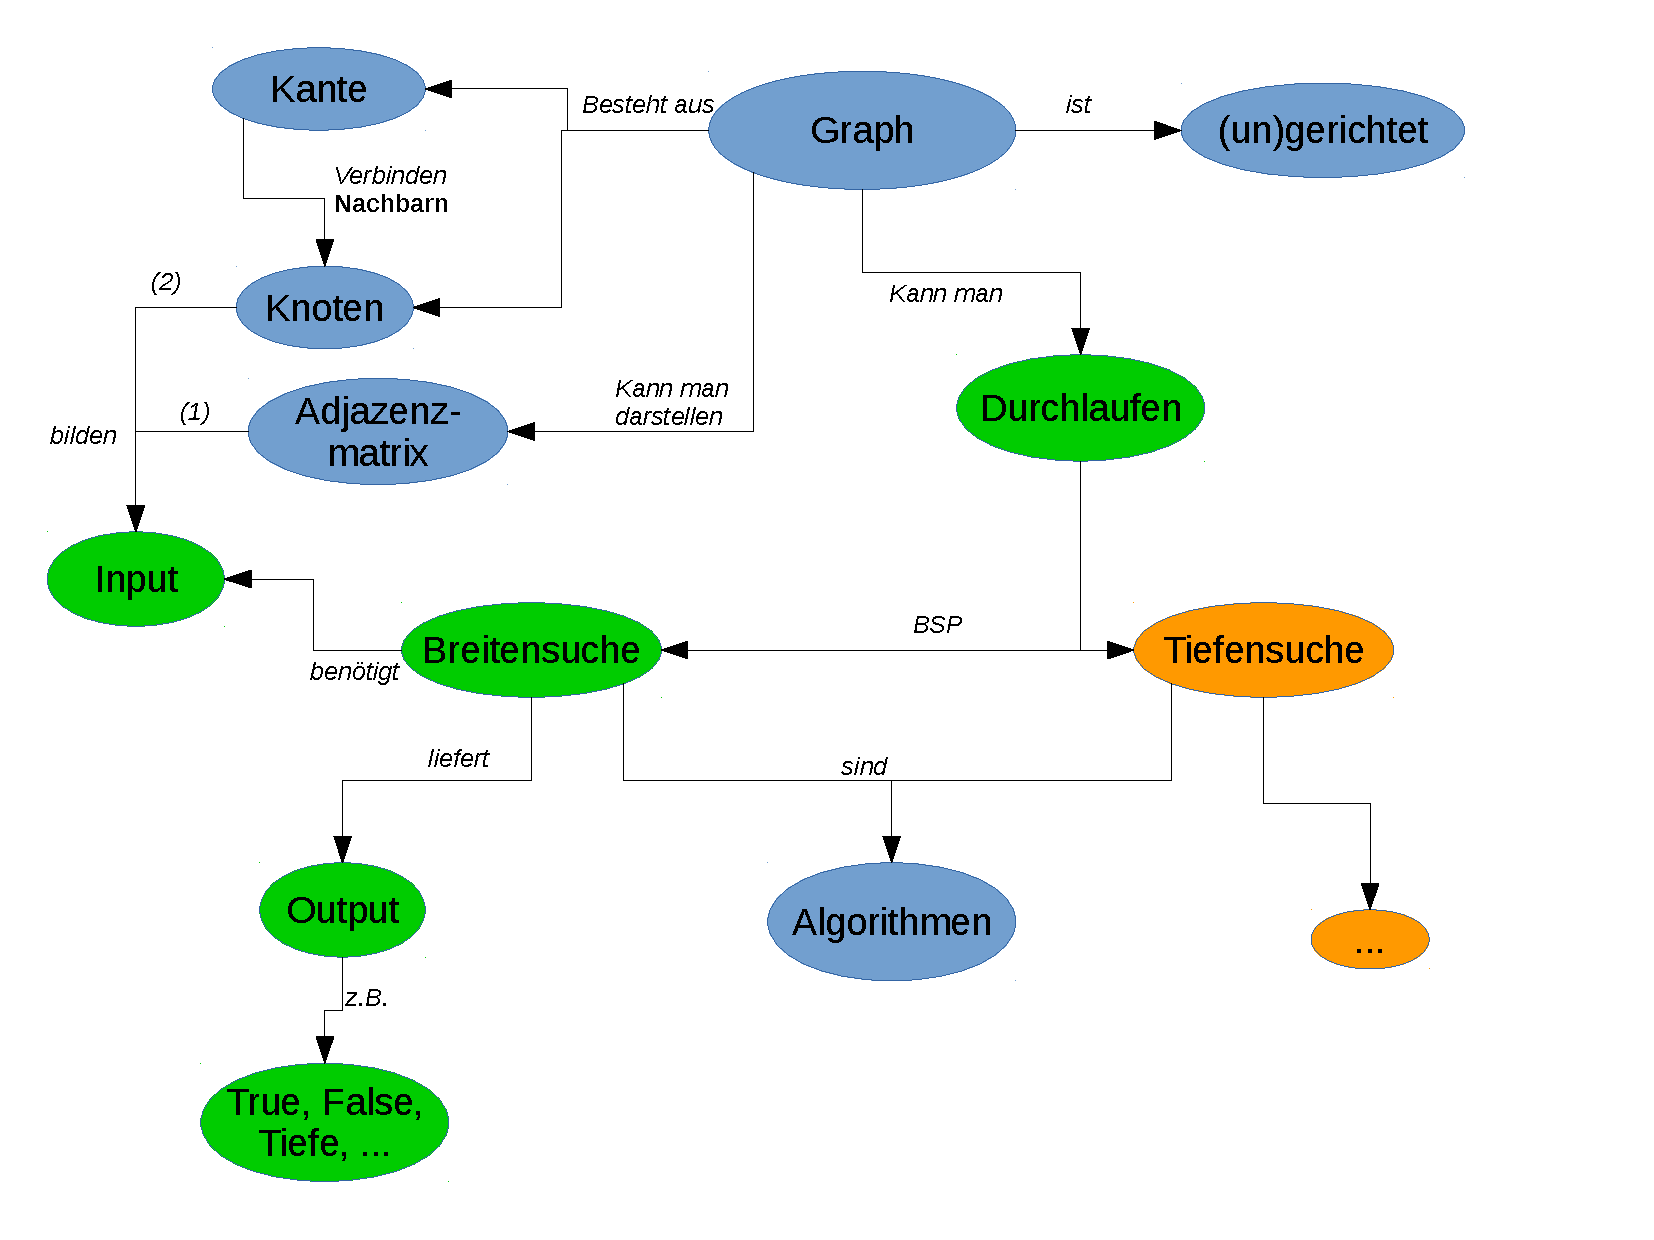
\includegraphics[width=.99\textwidth]{../cmap/bsuche_cmap.pdf}
%\caption{Concept-Map zum Thema Breitensuche.
%Blaue Konzepte bilden das Vorwissen ab. 
%Grüne Konzepte werden in dieser Arbeit eingeführt und behandelt. 
%Orangene Konzepte bilden einen Ausblick auf Konzepte, welche im Rahmen dieser Arbeit nicht mehr behandelt werden. 
%}
%\label{fig:cmap2}
%\end{center}
%\end{figure}

Haben Sie sich schon mal überlegt, wie Sie mithilfe des ÖV von einer Station zu ihrer Destination gelangen können. 
Zum Beispiel: Was ist die kürzeste Verbindung zwischen \emph{Hauptwil} und \emph{Horn} in St. Gallen (s. Abb.~\ref{fig:sbahn2}). 
Wahrscheinlich haben Sie sich auf der Website des Betreibers erkundigt und dort eine Antwort erhalten. 
Dies war eine automatisierte Bearbeitung Ihrer Anfrage und hinter Website steckt also ein Programm, dass mithilfe eines Algorithmus Ihre Anfrage bearbeitet und eine Ausgabe generiert.



\begin{figure}[htb]
\begin{center}

%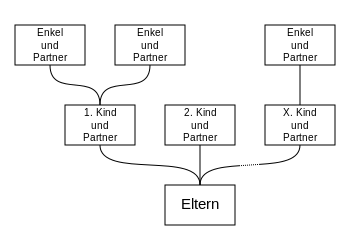
\includegraphics[width=.7\textwidth]{../fig/stammbaum.png}
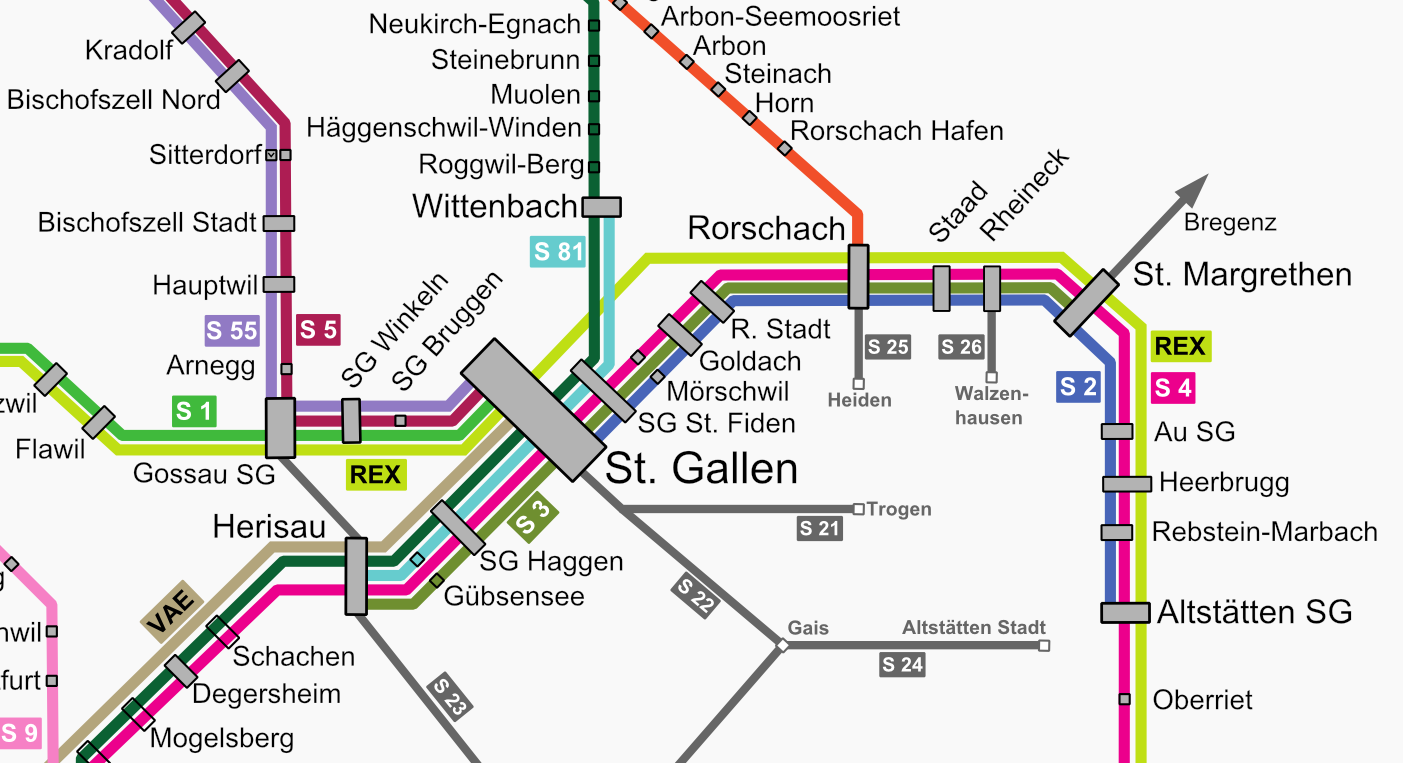
\includegraphics[width=.67\textwidth]{../fig/sbahn_netz_ausschnitt.png}
\caption{Darstellung eines Ausschnitts des Sankt Galler S-Bahn-Netzes als (ungerichteter) Graph.
Jede Station bildet dabei einen Knoten und die Verbindung zwischen den Knoten ist eine Kante.
%https://upload.wikimedia.org/wikipedia/commons/1/19/Map_S-Bahn_St._Gallen_%28schematic%29.png
}

\label{fig:sbahn2}
\end{center}
\end{figure}

Damit man aber das komplexe Gebilde eines Fahrplans für einen Algorithmus (Computerprogramm) vereinfachen kann, muss man sich auf eine Darstellung einigen. 
Jede Station eines Fahrplannetzes ist ein Knotenpunkt, von dem verschiedene Verbindungen zu  an deren Stationen ausgehen. 
Die mathematische Darstellung eines solchen Gebildes nennt man Graph.

Diesen Begriff haben Sie schon einmal kennengelernt und Sie wissen auch, dass man damit verschiedene Objekte mit einander verbinden kann. 
Eine interessante Frage ist immer, über wie viele Verbindungen zwei Objekte mit einander verknüpft sind. 
Wir möchten nun mit diesem Kapitel überlegen, wie man einen Graphen durchsuchen kann.
Ein Beispiel für einen solchen Algorithmus ist die Breitensuche. 
Ziel ist es, dass Sie den Algorithmus verstehen und anwenden können. 

%Der Aufbau dieses Kapitels ist so gehalten, dass Sie im ersten Abschnitt nochmal die Grundlagen zu Graphen wiederholen und festigen. 
%Dabei geht es vor allem um verschiedene Darstellungen von Graphen und das Konzept von Nachbarn.
%Im zweiten Abschnitt sollen dann Grundlagen des Modellierens von Problemen mit Hilfe von Graphen und das L\"osen der Probleme mit Hilfe von Algorithmen auf Graphen vermittelt werden.
%Insbesondere werden Problemstellungen betrachtet, die sich mit Hilfe eines neuen Algorithmus (\emph{Breitensuche}), lösen lassen. 
%Der Algorithmus für die Breitensuche wird dabei Schritt f\"ur Schritt erarbeitet, erweitert und implementiert.
%
%In der Concept-Map (s. Abb.~\ref{fig:cmap2}) können Sie die verschiedenen Konzepte und ihren Zusammenhang für das folgende Kapitel überblicken. 
%Mit der Farbe Blau markierte Konzepte sollten schon bekannt sein, aber werden nochmal wiederholt.
%Grün markiert sind neue Konzepte, die in dieser Einheit behandelt werden und orange sind Konzepte, die einen Ausblick bilden und nicht mehr behandelt werden. 

